% Options for packages loaded elsewhere
% Options for packages loaded elsewhere
\PassOptionsToPackage{unicode}{hyperref}
\PassOptionsToPackage{hyphens}{url}
\PassOptionsToPackage{dvipsnames,svgnames,x11names}{xcolor}
%
\documentclass[
  letterpaper,
  DIV=11,
  numbers=noendperiod]{scrartcl}
\usepackage{xcolor}
\usepackage{amsmath,amssymb}
\setcounter{secnumdepth}{-\maxdimen} % remove section numbering
\usepackage{iftex}
\ifPDFTeX
  \usepackage[T1]{fontenc}
  \usepackage[utf8]{inputenc}
  \usepackage{textcomp} % provide euro and other symbols
\else % if luatex or xetex
  \usepackage{unicode-math} % this also loads fontspec
  \defaultfontfeatures{Scale=MatchLowercase}
  \defaultfontfeatures[\rmfamily]{Ligatures=TeX,Scale=1}
\fi
\usepackage{lmodern}
\ifPDFTeX\else
  % xetex/luatex font selection
\fi
% Use upquote if available, for straight quotes in verbatim environments
\IfFileExists{upquote.sty}{\usepackage{upquote}}{}
\IfFileExists{microtype.sty}{% use microtype if available
  \usepackage[]{microtype}
  \UseMicrotypeSet[protrusion]{basicmath} % disable protrusion for tt fonts
}{}
\makeatletter
\@ifundefined{KOMAClassName}{% if non-KOMA class
  \IfFileExists{parskip.sty}{%
    \usepackage{parskip}
  }{% else
    \setlength{\parindent}{0pt}
    \setlength{\parskip}{6pt plus 2pt minus 1pt}}
}{% if KOMA class
  \KOMAoptions{parskip=half}}
\makeatother
% Make \paragraph and \subparagraph free-standing
\makeatletter
\ifx\paragraph\undefined\else
  \let\oldparagraph\paragraph
  \renewcommand{\paragraph}{
    \@ifstar
      \xxxParagraphStar
      \xxxParagraphNoStar
  }
  \newcommand{\xxxParagraphStar}[1]{\oldparagraph*{#1}\mbox{}}
  \newcommand{\xxxParagraphNoStar}[1]{\oldparagraph{#1}\mbox{}}
\fi
\ifx\subparagraph\undefined\else
  \let\oldsubparagraph\subparagraph
  \renewcommand{\subparagraph}{
    \@ifstar
      \xxxSubParagraphStar
      \xxxSubParagraphNoStar
  }
  \newcommand{\xxxSubParagraphStar}[1]{\oldsubparagraph*{#1}\mbox{}}
  \newcommand{\xxxSubParagraphNoStar}[1]{\oldsubparagraph{#1}\mbox{}}
\fi
\makeatother

\usepackage{color}
\usepackage{fancyvrb}
\newcommand{\VerbBar}{|}
\newcommand{\VERB}{\Verb[commandchars=\\\{\}]}
\DefineVerbatimEnvironment{Highlighting}{Verbatim}{commandchars=\\\{\}}
% Add ',fontsize=\small' for more characters per line
\usepackage{framed}
\definecolor{shadecolor}{RGB}{241,243,245}
\newenvironment{Shaded}{\begin{snugshade}}{\end{snugshade}}
\newcommand{\AlertTok}[1]{\textcolor[rgb]{0.68,0.00,0.00}{#1}}
\newcommand{\AnnotationTok}[1]{\textcolor[rgb]{0.37,0.37,0.37}{#1}}
\newcommand{\AttributeTok}[1]{\textcolor[rgb]{0.40,0.45,0.13}{#1}}
\newcommand{\BaseNTok}[1]{\textcolor[rgb]{0.68,0.00,0.00}{#1}}
\newcommand{\BuiltInTok}[1]{\textcolor[rgb]{0.00,0.23,0.31}{#1}}
\newcommand{\CharTok}[1]{\textcolor[rgb]{0.13,0.47,0.30}{#1}}
\newcommand{\CommentTok}[1]{\textcolor[rgb]{0.37,0.37,0.37}{#1}}
\newcommand{\CommentVarTok}[1]{\textcolor[rgb]{0.37,0.37,0.37}{\textit{#1}}}
\newcommand{\ConstantTok}[1]{\textcolor[rgb]{0.56,0.35,0.01}{#1}}
\newcommand{\ControlFlowTok}[1]{\textcolor[rgb]{0.00,0.23,0.31}{\textbf{#1}}}
\newcommand{\DataTypeTok}[1]{\textcolor[rgb]{0.68,0.00,0.00}{#1}}
\newcommand{\DecValTok}[1]{\textcolor[rgb]{0.68,0.00,0.00}{#1}}
\newcommand{\DocumentationTok}[1]{\textcolor[rgb]{0.37,0.37,0.37}{\textit{#1}}}
\newcommand{\ErrorTok}[1]{\textcolor[rgb]{0.68,0.00,0.00}{#1}}
\newcommand{\ExtensionTok}[1]{\textcolor[rgb]{0.00,0.23,0.31}{#1}}
\newcommand{\FloatTok}[1]{\textcolor[rgb]{0.68,0.00,0.00}{#1}}
\newcommand{\FunctionTok}[1]{\textcolor[rgb]{0.28,0.35,0.67}{#1}}
\newcommand{\ImportTok}[1]{\textcolor[rgb]{0.00,0.46,0.62}{#1}}
\newcommand{\InformationTok}[1]{\textcolor[rgb]{0.37,0.37,0.37}{#1}}
\newcommand{\KeywordTok}[1]{\textcolor[rgb]{0.00,0.23,0.31}{\textbf{#1}}}
\newcommand{\NormalTok}[1]{\textcolor[rgb]{0.00,0.23,0.31}{#1}}
\newcommand{\OperatorTok}[1]{\textcolor[rgb]{0.37,0.37,0.37}{#1}}
\newcommand{\OtherTok}[1]{\textcolor[rgb]{0.00,0.23,0.31}{#1}}
\newcommand{\PreprocessorTok}[1]{\textcolor[rgb]{0.68,0.00,0.00}{#1}}
\newcommand{\RegionMarkerTok}[1]{\textcolor[rgb]{0.00,0.23,0.31}{#1}}
\newcommand{\SpecialCharTok}[1]{\textcolor[rgb]{0.37,0.37,0.37}{#1}}
\newcommand{\SpecialStringTok}[1]{\textcolor[rgb]{0.13,0.47,0.30}{#1}}
\newcommand{\StringTok}[1]{\textcolor[rgb]{0.13,0.47,0.30}{#1}}
\newcommand{\VariableTok}[1]{\textcolor[rgb]{0.07,0.07,0.07}{#1}}
\newcommand{\VerbatimStringTok}[1]{\textcolor[rgb]{0.13,0.47,0.30}{#1}}
\newcommand{\WarningTok}[1]{\textcolor[rgb]{0.37,0.37,0.37}{\textit{#1}}}

\usepackage{longtable,booktabs,array}
\usepackage{calc} % for calculating minipage widths
% Correct order of tables after \paragraph or \subparagraph
\usepackage{etoolbox}
\makeatletter
\patchcmd\longtable{\par}{\if@noskipsec\mbox{}\fi\par}{}{}
\makeatother
% Allow footnotes in longtable head/foot
\IfFileExists{footnotehyper.sty}{\usepackage{footnotehyper}}{\usepackage{footnote}}
\makesavenoteenv{longtable}
\usepackage{graphicx}
\makeatletter
\newsavebox\pandoc@box
\newcommand*\pandocbounded[1]{% scales image to fit in text height/width
  \sbox\pandoc@box{#1}%
  \Gscale@div\@tempa{\textheight}{\dimexpr\ht\pandoc@box+\dp\pandoc@box\relax}%
  \Gscale@div\@tempb{\linewidth}{\wd\pandoc@box}%
  \ifdim\@tempb\p@<\@tempa\p@\let\@tempa\@tempb\fi% select the smaller of both
  \ifdim\@tempa\p@<\p@\scalebox{\@tempa}{\usebox\pandoc@box}%
  \else\usebox{\pandoc@box}%
  \fi%
}
% Set default figure placement to htbp
\def\fps@figure{htbp}
\makeatother


% definitions for citeproc citations
\NewDocumentCommand\citeproctext{}{}
\NewDocumentCommand\citeproc{mm}{%
  \begingroup\def\citeproctext{#2}\cite{#1}\endgroup}
\makeatletter
 % allow citations to break across lines
 \let\@cite@ofmt\@firstofone
 % avoid brackets around text for \cite:
 \def\@biblabel#1{}
 \def\@cite#1#2{{#1\if@tempswa , #2\fi}}
\makeatother
\newlength{\cslhangindent}
\setlength{\cslhangindent}{1.5em}
\newlength{\csllabelwidth}
\setlength{\csllabelwidth}{3em}
\newenvironment{CSLReferences}[2] % #1 hanging-indent, #2 entry-spacing
 {\begin{list}{}{%
  \setlength{\itemindent}{0pt}
  \setlength{\leftmargin}{0pt}
  \setlength{\parsep}{0pt}
  % turn on hanging indent if param 1 is 1
  \ifodd #1
   \setlength{\leftmargin}{\cslhangindent}
   \setlength{\itemindent}{-1\cslhangindent}
  \fi
  % set entry spacing
  \setlength{\itemsep}{#2\baselineskip}}}
 {\end{list}}
\usepackage{calc}
\newcommand{\CSLBlock}[1]{\hfill\break\parbox[t]{\linewidth}{\strut\ignorespaces#1\strut}}
\newcommand{\CSLLeftMargin}[1]{\parbox[t]{\csllabelwidth}{\strut#1\strut}}
\newcommand{\CSLRightInline}[1]{\parbox[t]{\linewidth - \csllabelwidth}{\strut#1\strut}}
\newcommand{\CSLIndent}[1]{\hspace{\cslhangindent}#1}



\setlength{\emergencystretch}{3em} % prevent overfull lines

\providecommand{\tightlist}{%
  \setlength{\itemsep}{0pt}\setlength{\parskip}{0pt}}



 


\usepackage{xspace}
\newcommand{\plyxp}{\textit{plyxp}\xspace}
\newcommand{\dplyr}{\textit{dplyr}\xspace}
\newcommand{\purrr}{\textit{purrr}\xspace}
\newcommand{\pandas}{\textit{pandas}\xspace}
\newcommand{\anndata}{\textit{AnnData}\xspace}
\newcommand{\rlang}{\textit{rlang}\xspace}
\newcommand{\airway}{\textit{airway}\xspace}
\newcommand{\matrixStats}{\textit{matrixStats}\xspace}
\newcommand{\tidyomics}{\textit{tidyomics}\xspace}
\newcommand{\tidyverse}{\textit{tidyverse}\xspace}
\newcommand{\tidySE}{\textit{tidySummarizedExperiment}\xspace}
\newcommand{\SE}{\textit{SummarizedExperiment}\xspace}
\newcommand{\PlySE}{\textit{PlySummarizedExperiment}\xspace}
\newcommand{\profvis}{\textit{profvis}\xspace}
\newcommand{\ggplot}{\textit{ggplot2}\xspace}
\newcommand{\SCE}{\textit{SingleCellExperiment}\xspace}

% also contexts
\newcommand{\assays}{\texttt{assays}\xspace}
\newcommand{\rows}{\texttt{rows}\xspace}
\newcommand{\cols}{\texttt{cols}\xspace}
\newcommand{\rowseval}{\texttt{rows(\dots)}\xspace}
\newcommand{\colseval}{\texttt{cols(\dots)}\xspace}
\newcommand{\dotenv}{\texttt{.env}\xspace}
\newcommand{\dotdata}{\texttt{.data}\xspace}
\newcommand{\dotrows}{\texttt{.rows}\xspace}
\newcommand{\dotcols}{\texttt{.cols}\xspace}
\newcommand{\dotassays}{\texttt{.assays}\xspace}
\newcommand{\asis}{\texttt{asis}\xspace}
\newcommand{\data}{\texttt{data}\xspace}

% functions
\newcommand{\mutate}{\texttt{mutate()}\xspace}
\newcommand{\filter}{\texttt{filter()}\xspace}
\newcommand{\groupby}{\texttt{group\_by()}\xspace}
\newcommand{\newplyxp}{\texttt{new\_plyxp()}\xspace}
\KOMAoption{captions}{tableheading}
\makeatletter
\@ifpackageloaded{caption}{}{\usepackage{caption}}
\AtBeginDocument{%
\ifdefined\contentsname
  \renewcommand*\contentsname{Table of contents}
\else
  \newcommand\contentsname{Table of contents}
\fi
\ifdefined\listfigurename
  \renewcommand*\listfigurename{List of Figures}
\else
  \newcommand\listfigurename{List of Figures}
\fi
\ifdefined\listtablename
  \renewcommand*\listtablename{List of Tables}
\else
  \newcommand\listtablename{List of Tables}
\fi
\ifdefined\figurename
  \renewcommand*\figurename{Figure}
\else
  \newcommand\figurename{Figure}
\fi
\ifdefined\tablename
  \renewcommand*\tablename{Table}
\else
  \newcommand\tablename{Table}
\fi
}
\@ifpackageloaded{float}{}{\usepackage{float}}
\floatstyle{ruled}
\@ifundefined{c@chapter}{\newfloat{codelisting}{h}{lop}}{\newfloat{codelisting}{h}{lop}[chapter]}
\floatname{codelisting}{Listing}
\newcommand*\listoflistings{\listof{codelisting}{List of Listings}}
\makeatother
\makeatletter
\makeatother
\makeatletter
\@ifpackageloaded{caption}{}{\usepackage{caption}}
\@ifpackageloaded{subcaption}{}{\usepackage{subcaption}}
\makeatother
\usepackage{bookmark}
\IfFileExists{xurl.sty}{\usepackage{xurl}}{} % add URL line breaks if available
\urlstyle{same}
\hypersetup{
  colorlinks=true,
  linkcolor={blue},
  filecolor={Maroon},
  citecolor={Blue},
  urlcolor={Blue},
  pdfcreator={LaTeX via pandoc}}


\author{}
\date{}
\begin{document}


\section{Introduction}\label{introduction}

High-throughput omics data are often summarized into one or more
matrices representing counts or relative abundance of molecules in a set
of experiments, as summarized across various genomic features (rows),
and across different experiments or samples (columns). During subsequent
analysis, it is critical to preserve links between rows and columns of
the matrix data with relevant feature and sample metadata tables. For
example, one may wish to divide a matrix of RNA-seq transcript counts by
the transcript length (metadata associated with the transcript features
along the rows) or by the library size (metadata associated with samples
along the columns). This need for robust and efficient handling of
annotated matrix data motivated the development of various data classes,
including but not limited to the \emph{ExpressionSet} (Gentleman et al.
2004) and the \emph{SummarizedExperiment} (Huber et al. 2015) in
R/Bioconductor, and \emph{AnnData} (Virshup et al. 2024) in Python. Such
annotated matrix data classes and associated methods ensure that
structural consistency is maintained between data and metadata during
common operations such as subsetting, re-ordering, and row or column
binding.

Operating on these data objects requires learning domain-specific
functions and syntax. Performing complex operations such as grouping
over sets of rows and columns and computing further data summarization
may require writing additional control structures such as for loops or
using less well-known functional programming helpers, which can
obfuscate the purpose of analysis code. The \emph{tidyomics} project was
created within R/Bioconductor to help address this issue (Hutchison et
al. 2024), providing methods and coding paradigms for working with
common R data classes representing genomic ranges (Lee, Cook, and
Lawrence 2019; Lee, Lawrence, and Love 2020), count matrices (Mangiola
et al. 2021), and Seurat objects (Mangiola, Doyle, and Papenfuss 2021).
The project enables intuitive manipulation and visualization without
requiring users to learn domain-specific syntax. \emph{tidyomics}
packages and workflows enable chained data-manipulative operations that
resemble the style and framework of tidy data analysis (Wickham 2014) as
implemented in \emph{dplyr} (Wickham et al. 2023) and other
\emph{tidyverse} (Wickham et al. 2019) packages, or chained operations
for python \emph{DataFrames} using \emph{pandas} (McKinney 2022). Due to
the popularity of the \emph{tidyverse} among newer R users,
\emph{tidyomics} increases the accessibility of omic data analysis.

Here, we propose a new expressive grammar for access and manipulation of
annotated matrix data and a framework for efficiently performing the
operations implied by the syntax. Data within the annotated matrix
object are lazily bound to a series of environments that are evaluated
when the user forces their symbols. Thus, a user has more freedom in how
they choose to work with their data. We introduce the \emph{plyxp} R
package that implements this grammar, allowing the use of \emph{dplyr}
syntax with the Bioconductor \emph{SummarizedExperiment} (SE) data
class.

The \emph{tidySummarizedExperiment} package, which was released with
Bioconductor 3.12 in 2020, also provides \emph{dplyr}-like access to SE
objects within the \emph{tidyomics} project. The
\emph{tidySummarizedExperiment} package allows users to approach the SE
as an abstracted data frame, conceptually unwrapping the compact matrix
representation into a tidy, long-form version.
\emph{tidySummarizedExperiment} facilitates data exploration and
visualization, allowing datasets to be directly piped into \emph{ggplot}
plotting functions.

However some complex computations involving simultaneous manipulation of
matrix values and annotation metadata were slower than necessary, a
limitation addressable through data-masking strategies.

\emph{plyxp}'s use of data masking from the \emph{rlang} (Henry and
Wickham 2026) package provides gains in efficiency and is currently used
to speed up existing functionality within
\emph{tidySummarizedExperiment}.

Further, \emph{plyxp} reinforces the structure of the annotated matrix
through additional syntax compared to \emph{tidySummarizedExperiment},
often resulting in more verbose, but more specific evaluation.

\section{Syntax}\label{syntax}

We describe a grammar in which users can access, modify, and append data
across different contexts of a dataset, where here we mean ``context''
to refer to a collection of objects of the same length (for vectors) or
dimension (for matrices), which collectively describe either features,
samples, or a matrix of values over features and samples. For annotated
matrix data with \(n\) rows and \(p\) columns, we define three contexts:
the \texttt{assays} consist of one or more matrices of size
\(n \times p\); the \texttt{rows} consist of row metadata (a collection
of vectors of length \(n\) describing the features); and the
\texttt{cols} consist of column metadata (a collection of vectors of
length \(p\) describing the samples/cells). For example, an object
representing an RNA-seq experiment might have an \texttt{assays} context
consisting of a counts matrix and a transcripts-per-million (TPM) matrix
across \(n\) genes and \(p\) samples, a \texttt{rows} context with
feature metadata such as alternative gene identifiers and gene length,
and a \texttt{cols} context with sample metadata such as library size
and sample condition group.

By default, expressions are evaluated against the named symbols within
the \texttt{assays} context. The user can specify to evaluate against
named symbols in the row or column metadata by decorating their
expressions with sentinel functions, \texttt{r\ rows(...)} or
\texttt{r\ cols(...)}. Beyond communicating where expressions are
evaluated, this syntax also enforces where the resulting vector or
matrix will be stored. For example, with the \texttt{r\ mutate()}
command, the new objects are bound to their respective context within
the object, but for the \texttt{r\ filter()} command, instead of adding
data, these results inform how the rows or columns should be subset.

\begin{Shaded}
\begin{Highlighting}[]
\NormalTok{data }\SpecialCharTok{|\textgreater{}}
  \FunctionTok{mutate}\NormalTok{(}
    \AttributeTok{log10\_counts =} \FunctionTok{log10}\NormalTok{(counts }\SpecialCharTok{+} \DecValTok{1}\NormalTok{),}
    \FunctionTok{cols}\NormalTok{(}\AttributeTok{treated =}\NormalTok{ (dex }\SpecialCharTok{==} \StringTok{"trt"}\NormalTok{))}
\NormalTok{  )}
\end{Highlighting}
\end{Shaded}

\begin{Shaded}
\begin{Highlighting}[]
\NormalTok{data }\SpecialCharTok{|\textgreater{}}
  \FunctionTok{filter}\NormalTok{(}
    \FunctionTok{rows}\NormalTok{(gene\_biotype }\SpecialCharTok{==} \StringTok{"lincRNA"}\NormalTok{),}
    \FunctionTok{cols}\NormalTok{(avgLength }\SpecialCharTok{\textgreater{}=} \DecValTok{126}\NormalTok{)}
\NormalTok{  )}
\end{Highlighting}
\end{Shaded}

The above example demonstrates this grammar as implemented in
\emph{plyxp}.

The user computes the logarithm of the counts matrix plus a pseudocount,
and creates a new logical variable in the column metadata, each of which
are stored in their respective contexts. In the next step of the pipe,
rows and columns are filtered based on available metadata about the
genes and the samples. Here the base R \texttt{\textbar{}\textgreater{}}
symbol refers to piping the results of a function into the first place
argument of the following function. As in \emph{dplyr}, the
\texttt{mutate()} verb implies an addition of an object (matrix or
vector) to the corresponding evaluation context, whereas
\texttt{filter()} subsets the data (described more later).

The \emph{plyxp} syntax is designed to be convenient and flexible,
providing users with multiple tools to access or manipulate their data
across contexts. For example, consider the following:

\begin{Shaded}
\begin{Highlighting}[]
\NormalTok{data }\SpecialCharTok{|\textgreater{}}
  \FunctionTok{mutate}\NormalTok{(}
    \AttributeTok{norm\_cts =}\NormalTok{ counts}\SpecialCharTok{/}\NormalTok{.cols}\SpecialCharTok{$}\NormalTok{size\_factor,}
    \AttributeTok{cts\_bp =}\NormalTok{ counts}\SpecialCharTok{/}\NormalTok{.rows}\SpecialCharTok{$}\NormalTok{gene\_length}
\NormalTok{  )}
\end{Highlighting}
\end{Shaded}

Using pronouns \texttt{.cols} and \texttt{.rows}, the user accesses
vectors from another context. A ``pronoun'' is a special object of the
\emph{rlang} package that provides an unambiguous symbol lookup into
named lists or environments. In the above expression, an element-wise
division of the counts matrix via data within the columns or rows is
done by replicating the data to the appropriate size automatically.

Alternatively, in the computation of \texttt{gene\_ave} in the following
code chunk, the user employs the efficient row-wise means operator
\texttt{rowMeans}. Alternatively, for \texttt{gene\_ave2} the expression
\texttt{.assays\$counts} within the row context is resolved to a list
where each element is a row of the counts matrix. A list output for the
\texttt{.assays} pronoun offers flexibility as lists can be supplied to
the apply family of functions or using \emph{purrr} (Wickham and Henry
2025) as shown below.

\begin{Shaded}
\begin{Highlighting}[]
\NormalTok{data }\SpecialCharTok{|\textgreater{}}
  \FunctionTok{mutate}\NormalTok{(}
    \FunctionTok{rows}\NormalTok{(}
      \AttributeTok{gene\_ave =} \FunctionTok{rowMeans}\NormalTok{(.assays\_asis}\SpecialCharTok{$}\NormalTok{counts),}
      \AttributeTok{gene\_ave2 =} \FunctionTok{map\_dbl}\NormalTok{(.assays}\SpecialCharTok{$}\NormalTok{counts, mean)}
\NormalTok{    )}
\NormalTok{  )}
\end{Highlighting}
\end{Shaded}

In the example code above, the \texttt{data} object can be instantiated
from any \emph{SummarizedExperiment} using the \texttt{r\ new\_plyxp()}
function (see Supplementary Note for more details).

\section{Semantics}\label{semantics}

\emph{plyxp} is an implementation of this grammar for annotated matrix
data stored in R/Bioconductor's \emph{SummarizedExperiment} class,
allowing the use of \emph{dplyr} verbs with the following expected
outcomes and behaviors. \emph{plyxp} enforces conventions that eliminate
ambiguity while providing flexibility in terms of data shape and
computation:

\begin{enumerate}
\def\labelenumi{\arabic{enumi}.}
\tightlist
\item
  Expressions are scoped explicitly to an evaluation context.
\item
  Evaluation contexts are connected via pronouns, which provide both an
  \texttt{asis} and size-stable version of the requested data.
\item
  \emph{dplyr} verbs (\texttt{r\ mutate()}, \texttt{r\ filter()}, etc.)
  only support expressions that would result in the same structure of
  object as input (SE object).
\end{enumerate}

Evaluation contexts and their connection via pronouns are diagrammed in
Figure \textbf{?@fig-plyxp-diagram}. We note that \emph{plyxp} relies on
Bioconductor-native calls, e.g.~subsetting with square brackets
\texttt{{[},{]}}, and is thus never faster than using the SE interface
directly. There will always be some overhead in generating the necessary
abstraction to enable implicit references into the object as required by
\emph{dplyr}. However, we aim that \emph{plyxp} always be as close to
Bioconductor-native speed as possible, via line profiling of the
function definitions using \emph{profvis}.

\subsection{Pronouns and Data Masks}\label{pronouns-and-data-masks}

\emph{plyxp} enables expressive evaluation by leveraging \emph{rlang}
data masks, a series of basic R environments that are evaluated with the
\emph{rlang} tidy evaluation engine Wickham (2019). \emph{plyxp}
exploits several utilities from the \emph{rlang} package, such as lazy
evaluation and \emph{rlang} pronouns, to manage these environments.
Here, ``lazy evaluation'' refers to expressions whose computation is
delayed until the value is accessed. A developer may choose any number
of environments for their data mask that are necessary for their use
case. With multi-context scenarios that require multiple data masks, as
with annotated matrix data, we suggest the final parent ancestor
environment of the mask is reserved for binding \emph{rlang} pronouns.
This suggestion is motivated by R's lexical scoping, which allows
variable bindings to be searched through environment parents during
evaluation (R Core Team 2025). Placing pronouns in the final parent of
the mask, \emph{i.g.} the final environment prior to the calling
environment, will ensure the user's data within the context are
prioritized over potential access to other contexts. The \emph{rlang}
pronouns can be conceptually thought of as a pointer to another
environment. \emph{rlang} pronouns are utilized within the \emph{dplyr}
package to disambiguate where to find a symbol, in either the calling
environment or user's data with \texttt{.env}and\texttt{.data} pronouns
respectively.

In \emph{plyxp}, these pronouns are used to connect each context through
two pronouns, an \texttt{asis} variant and a
`\texttt{size-stable\textquotesingle{}\textquotesingle{}\ variant.\ The}asis\texttt{variant\ is\ to\ provide\ the\ user\ with\ access\ to\ the\ actual\ data\ stored\ on\ the\ object,\ as\ there\ may\ be\ efficient\ ways\ to\ operate\ on\ its\ native\ shape\ \_e.g.\_\ the\ row-wise\ and\ column-wise\ matrix\ operations\ in\ base\ R\ and\ \_matrixStats\_.\ The\ size-stable\ variant\ provides\ the\ requested\ data\ reshaped\ to\ match\ the\ size\ of\ the\ current\ context.\ The\ size-stable\ variant\ is\ intended\ to\ reduce\ friction\ from\ pulling\ data\ from\ other\ contexts,\ as\ there\ is\ no\ guarantee\ the\ target\ data}asis`
will match the expected output size of the evaluation context.

With annotated matrix data, there are predictable transformations that
may be used to guarantee size stability. For example, consider
requesting row or column data from within the \texttt{assays} evaluation
context. To make the row data size stable, we need only to replicate the
target vector as many times as the number of columns in our matrix
context, and then concatenate these vectors. For column data within the
\texttt{assays} evaluation context, we replicate each element of the
target vector as many times as the number of rows in our matrix context.
Requesting assay data from within the \texttt{rows} or \texttt{cols}
evaluation context, we may reshape the matrix by returning a list where
each element is a row or column of the matrix, respectively.

\pandocbounded{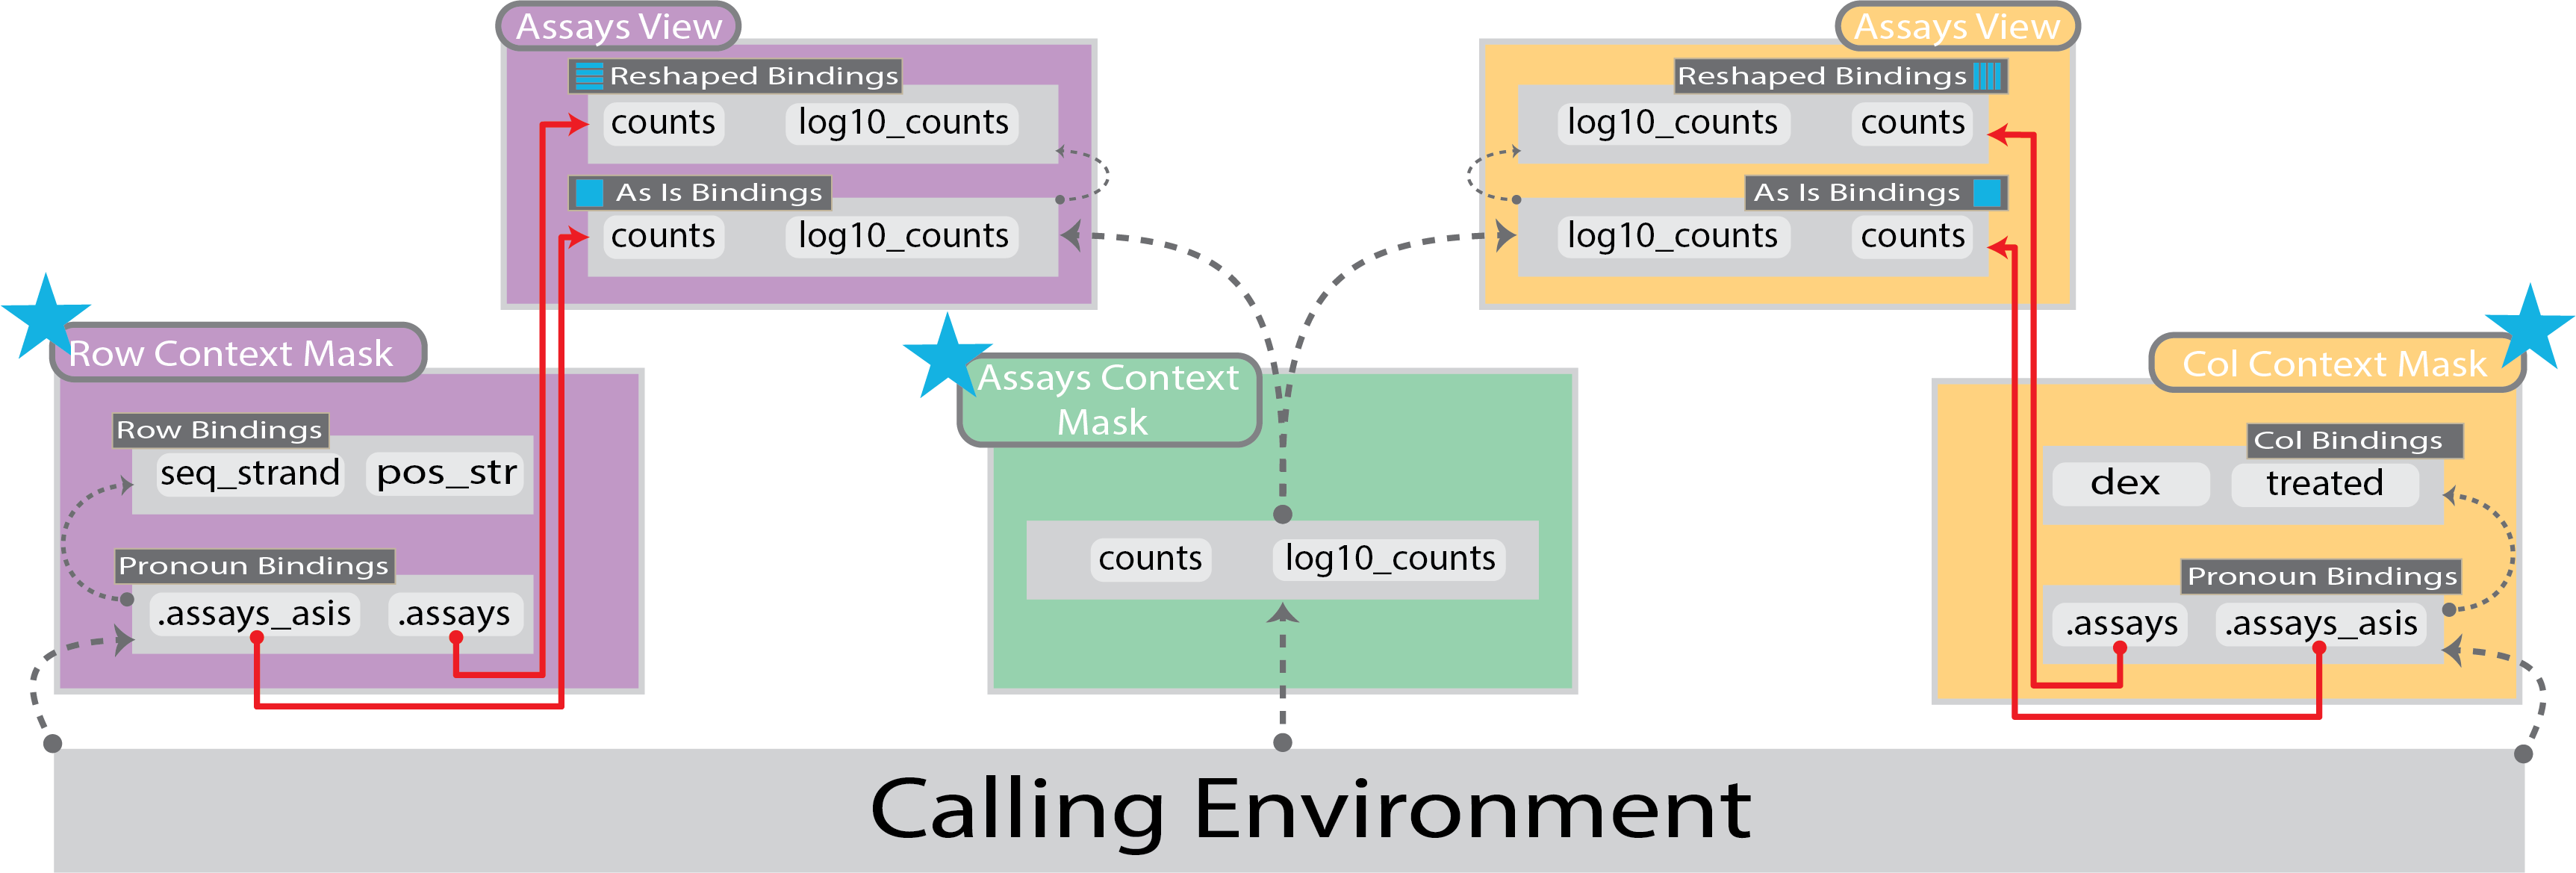
\includegraphics[keepaspectratio]{./application_note_F1_005.png}}\{\#fig-plyxp-diagram
, width=``textwidth''\}

\subsection{Grouping}\label{grouping}

In \emph{dplyr}, specifying groups with \texttt{r\ group\_by()} augments
the behavior of further \emph{dplyr} verbs. \emph{dplyr} grouping
operations traditionally include additional metadata on the target
object describing how the data should be partitioned. This strategy
works well for data structures that are rectangular, but may lead to
ambiguities for data structures that deviate from this structure, such
as annotated matrix data. For tabular data, there is only one dimension
(along the rows) in which those data can be partitioned, and no matter
how the rows are partitioned, a new table can be constructed from the
results. This is not true for matrices. One such example would be to
attempt to group by matrix values \textgreater{} 100. Here, there is no
guarantee the partitioning of arbitrary elements of a matrix would
create valid sub-matrices. It is for this reason that \emph{plyxp}
follows strict heuristics for grouping and only allows groupings that
partition rows or columns of the matrix.

This restriction coincides with the natural extension of applying
grouping to tabular data from \emph{dplyr}. We may conceptually regard
the row data and the column data as independent and grouped as normal
tabular structures. The row data and the column data are related to one
another through the matrix, and thus the matrix observes all grouping
partitions imposed on both dimensions. Since the row data and the column
data groupings are independent, the \texttt{rows} and \texttt{cols}
contexts only consider their own respective grouping during evaluation.
In other words, the \texttt{assays} context will always respect
groupings about the \texttt{rows} and \texttt{cols} contexts, but the
\texttt{rows} context drops any \texttt{cols} grouping and \texttt{cols}
context drops any \texttt{rows} grouping.

\section{Performance Comparison}\label{performance-comparison}

All evaluation within \emph{plyxp} is intended to take place within one
of the specified contexts mentioned previously. Due to the particular
shape of annotated matrix data, each context has a unique notion of size
and a unique set of symbols within. Additional syntax is used to declare
where an expression evaluates and there is no additional cost to
accessing data \texttt{asis}. An alternative to this approach would be
to force all variables within the same context, such as an instantiated
or abstracted \emph{data.frame} where all contexts are joined together.

A single context would require variables within the assays to be unwound
into one dimensional vectors, and data within the row and column
metadata tables to be replicated appropriately. Additional performance
considerations are discussed in more detail in the supplemental note.
When comparing between the two approaches, namely \emph{plyxp} compared
to annotated matrix data unwound into a \emph{data.frame}, \emph{plyxp}
runs \(\sim 14\) times faster when scaling the counts matrix by gene
length using the \emph{airway} dataset (Himes et al. 2014).

\section{Conclusion}\label{conclusion}

\emph{plyxp} provides a framework for operating on annotated matrix
data. As data masking was possible via the \emph{rlang} package, we were
able to introduce novel syntax for operating on SE objects within
Bioconductor that is ergonomically inspired by \emph{dplyr} style and
unambiguously expressive. \emph{tidySummarizedExperiment} has
incorporated \emph{plyxp} methods internally for some operations as of
Bioconductor 3.22 release in Fall 2025, such that users of both
\emph{plyxp} and \emph{tidySummarizedExperiment} benefit from the
performance gains described above, as compared to operations that would
require creation of a long form tabular representation of the annotated
matrix data. We imagine that the grammar described here could be applied
to manipulate \emph{AnnData} with \emph{pandas} methods. We plan to
release the internals of \emph{plyxp} that construct and manage the data
masks so that developers can choose to create their own \emph{dplyr}
style for additional R classes.

\section{Code Availability}\label{code-availability}

The \emph{plyxp} software package is available from Bioconductor,
installable with \texttt{BiocManager::install()}, and at
\url{https://github.com/jtlandis/plyxp}. All code used in this paper,
including comparisons of run time to alternative implementations and
reproducible code chunks appearing above, is available at
\url{https://github.com/jtlandis/plyxp_paper}

\newpage

\phantomsection\label{refs}
\begin{CSLReferences}{1}{0}
\bibitem[\citeproctext]{ref-Gentleman2004}
Gentleman, Robert C, Vincent J Carey, Douglas M Bates, Ben Bolstad,
Marcel Dettling, Sandrine Dudoit, Byron Ellis, et al. 2004.
{``Bioconductor: Open Software Development for Computational Biology and
Bioinformatics.''} \emph{Genome Biology} 5 (10): R80.

\bibitem[\citeproctext]{ref-rlang}
Henry, Lionel, and Hadley Wickham. 2026. \emph{Rlang: Functions for Base
Types and Core r and 'Tidyverse' Features}.
\url{https://doi.org/10.32614/CRAN.package.rlang}.

\bibitem[\citeproctext]{ref-Himes2014}
Himes, Blanca E, Xiaofeng Jiang, Peter Wagner, Ruoxi Hu, Qiyu Wang,
Barbara Klanderman, Reid M Whitaker, et al. 2014. {``{RNA-Seq}
Transcriptome Profiling Identifies {CRISPLD2} as a Glucocorticoid
Responsive Gene That Modulates Cytokine Function in Airway Smooth Muscle
Cells.''} \emph{PLOS One} 9 (6): e99625.

\bibitem[\citeproctext]{ref-Huber2015}
Huber, Wolfgang, Vincent J Carey, Robert Gentleman, Simon Anders, Marc
Carlson, Benilton S Carvalho, Hector Corrada Bravo, et al. 2015.
{``Orchestrating High-Throughput Genomic Analysis with Bioconductor.''}
\emph{Nature Methods} 12 (2): 115--21.

\bibitem[\citeproctext]{ref-Hutchison2024}
Hutchison, William J, Timothy J Keyes, tidyomics Consortium, Helena L
Crowell, Jacques Serizay, Charlotte Soneson, Eric S Davis, et al. 2024.
{``The Tidyomics Ecosystem: Enhancing Omic Data Analyses.''}
\emph{Nature Methods} 21 (7): 1166--70.

\bibitem[\citeproctext]{ref-Lee2019}
Lee, Stuart, Dianne Cook, and Michael Lawrence. 2019. {``Plyranges: A
Grammar of Genomic Data Transformation.''} \emph{Genome Biology} 20 (1):
4. \url{https://doi.org/10.1186/s13059-018-1597-8}.

\bibitem[\citeproctext]{ref-Lee2020}
Lee, Stuart, Michael Lawrence, and Michael I Love. 2020. {``Fluent
Genomics with Plyranges and Tximeta.''} \emph{F1000Res.} 9 (February):
109.

\bibitem[\citeproctext]{ref-Mangiola2021Seurat}
Mangiola, Stefano, Maria A Doyle, and Anthony T Papenfuss. 2021.
{``Interfacing Seurat with the {R} Tidy Universe.''}
\emph{Bioinformatics} 37 (22): 4100--4107.

\bibitem[\citeproctext]{ref-Mangiola2021bulk}
Mangiola, Stefano, Ramyar Molania, Ruining Dong, Maria A Doyle, and
Anthony T Papenfuss. 2021. {``Tidybulk: An {R} Tidy Framework for
Modular Transcriptomic Data Analysis.''} \emph{Genome Biol.} 22 (1): 42.

\bibitem[\citeproctext]{ref-McKinney2022}
McKinney, Wes. 2022. \emph{Python for Data Analysis 3e}. 3rd ed.
Sebastopol, CA: O'Reilly Media.

\bibitem[\citeproctext]{ref-rbase}
R Core Team. 2025. \emph{R: A Language and Environment for Statistical
Computing}. Vienna, Austria: R Foundation for Statistical Computing.
\url{https://www.R-project.org/}.

\bibitem[\citeproctext]{ref-Virshup2024}
Virshup, Isaac, Sergei Rybakov, Fabian J. Theis, Philipp Angerer, and F.
Alexander Wolf. 2024. {``Anndata: Access and Store Annotated Data
Matrices.''} \emph{Journal of Open Source Software} 9 (101): 4371.
\url{https://doi.org/10.21105/joss.04371}.

\bibitem[\citeproctext]{ref-Wickham2014}
Wickham, Hadley. 2014. {``Tidy Data.''} \emph{Journal of Statistical
Software} 59 (10): 1--23. \url{https://doi.org/10.18637/jss.v059.i10}.

\bibitem[\citeproctext]{ref-Wickham2019}
---------. 2019. \emph{Advanced r, Second Edition}. 2nd ed. Chapman \&
Hall/CRC the r Series. Philadelphia, PA: Chapman \& Hall/CRC.

\bibitem[\citeproctext]{ref-tidyverse}
Wickham, Hadley, Mara Averick, Jennifer Bryan, Winston Chang, Lucy
D'Agostino McGowan, Romain François, Garrett Grolemund, et al. 2019.
{``Welcome to the {tidyverse}.''} \emph{Journal of Open Source Software}
4 (43): 1686. \url{https://doi.org/10.21105/joss.01686}.

\bibitem[\citeproctext]{ref-dplyr}
Wickham, Hadley, Romain François, Lionel Henry, Kirill Müller, and Davis
Vaughan. 2023. \emph{Dplyr: A Grammar of Data Manipulation}.
\url{https://doi.org/10.32614/CRAN.package.dplyr}.

\bibitem[\citeproctext]{ref-purrr}
Wickham, Hadley, and Lionel Henry. 2025. \emph{Purrr: Functional
Programming Tools}. \url{https://doi.org/10.32614/CRAN.package.purrr}.

\end{CSLReferences}




\end{document}
